\chapter{Application: molécules et poches d'eau}

\boitemagique{Objectif}{
Lors de ce chapitre nous montrons que MDFT est capable de retrouver les molécules d'eau résolues expérimentalements, ainsi que les poches à l'intérieur des protéines.
}

Dans les chapitres précedents, nous avons montré la façon dont nous avons préparé MDFT afin de permettre l'étude de systèmes biologiques. Nous allons ici présenter deux exemples d'applications dans ce domaine. La première concerne la prédiction de la structure de solvatation alors que la seconde est une comparaison des énergies libres de solvatation calculées par MDFT et via une méthode implicite MM-PBSA.


\section{application 1: Peut on retrouver les molécules d'eau crystallographiques?}
Certaines molécules d'eau jouent un rôle important dans les intéractions et la stabilisation de système biologiques. Ces molécules ditent "fixes" sont généralement liées à nos système biologiques via de fortes intéractions: les liaisons Hydrogènes. Cette fixation bloque toute mobilité de ces molécules ce qui permet de les observer expérimentalement. En d'autre termes, ces molécules sont observables car leur probabilité de présence est forte. Ces molécules doivent donc se trouver dans des zones de fortes densité prédites par MDFT.
Dans cette partie, nous comparons dans un premier temps, les résultats obtenus par MDFT et ceux obtenus par dynamique moléculaire, notre référence. Dans un deuxième temps nous vérifions l'adéquation entre les zones de forte probabilité de présence fournies par ces deux méthodes et la position des molécules d'eau expérimentales.




\subsection{Les molécules}
Afin de mener cette étude, deux protéines ont été selectionnées. La première est une \textit{Streptomyces Erythraeus Trypsin} composée de 227 acides aminés. Cette protéine issue de la PDB [lien pdb] sous le code 4M7G à été selectionnée pour la qualité de sa résolution espérimentale (0.81 \AA).
La seconde est une \textit{FACTOR XA} composée de 241 acides aminés. Cette protéine issue de la PDB [lien pdb] sous le code 1HCG à été selectionnée car elle représente un permier cas d'étude simple, sans ligand ni contre ions.

\begin{center}
	\fbox{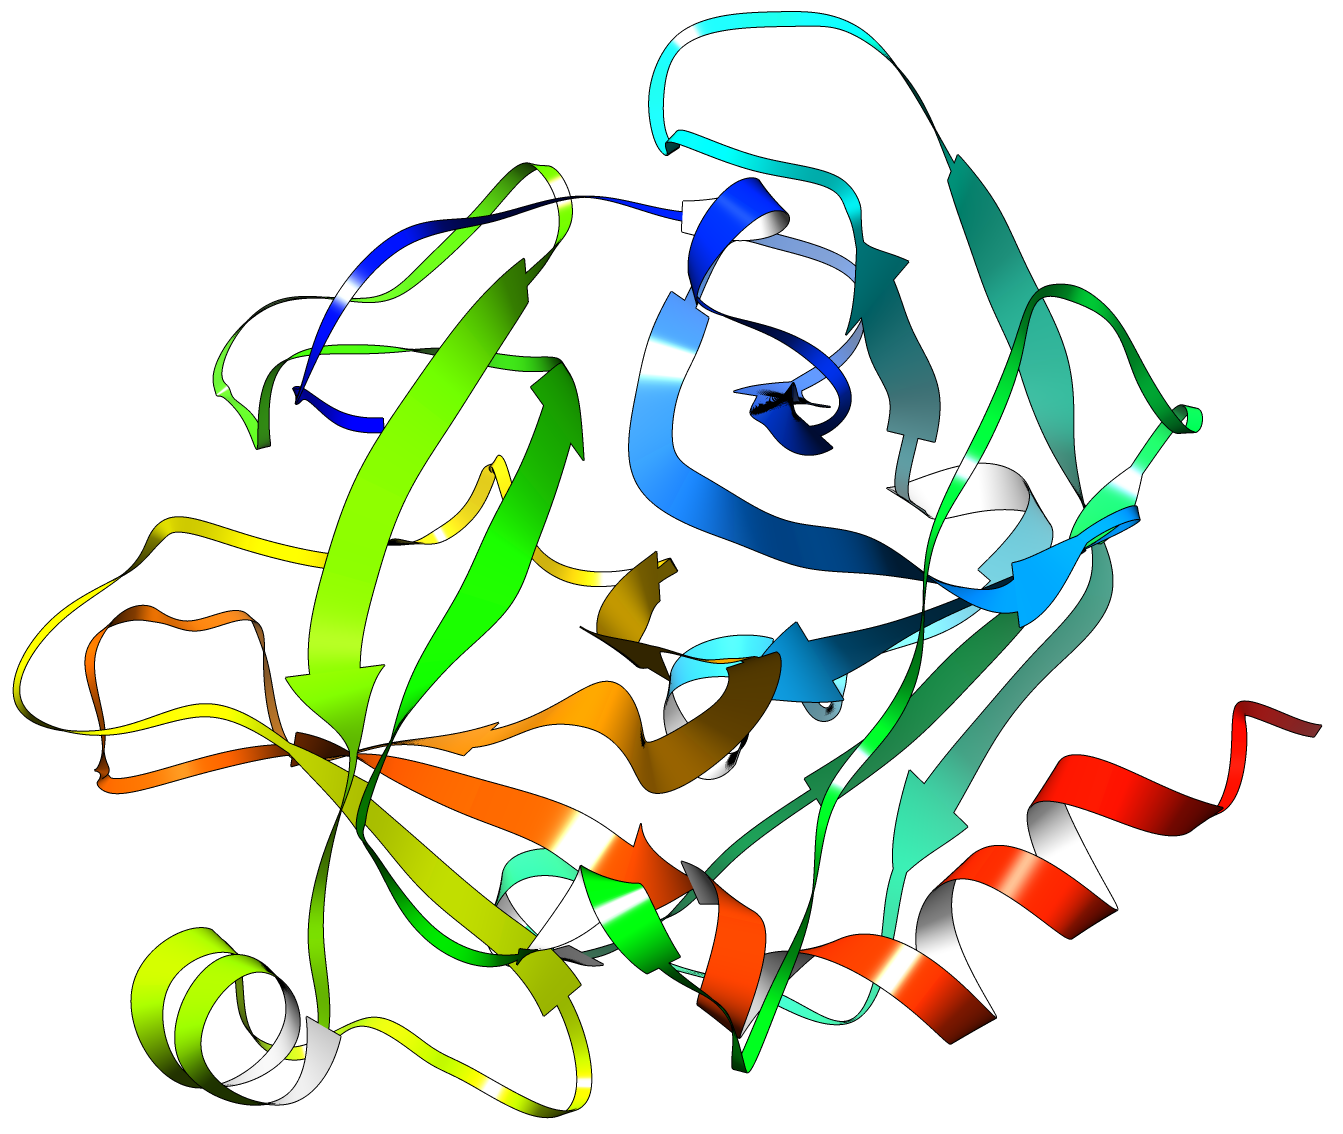
\includegraphics[width=\textwidth]{images/4m7g.png}}
	\captionof{figure}{Représentation en structure secondaire de la protéine 4M7G. Image réalisée en utilisant chimera [lien vers chimera]}
\end{center}


\begin{center}
	\fbox{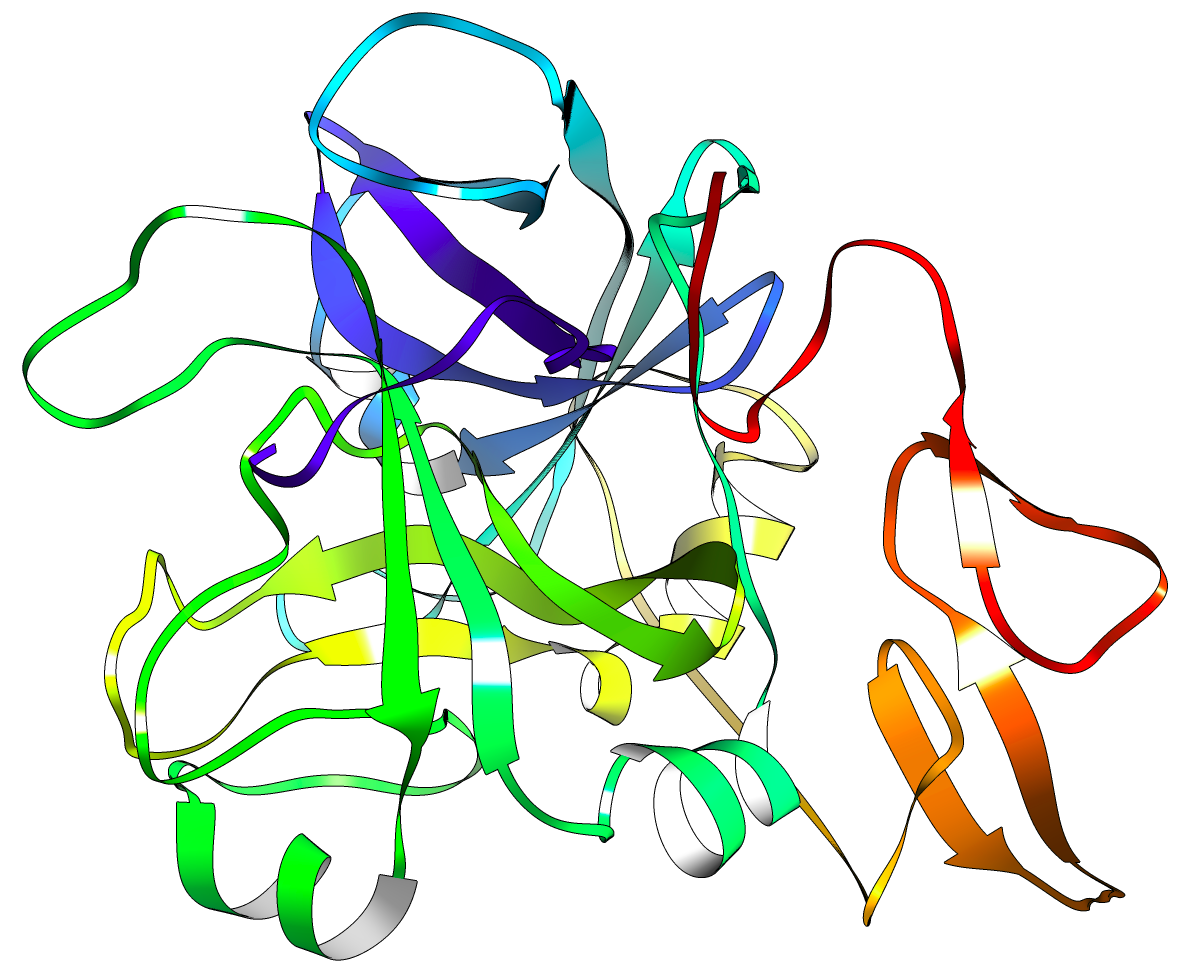
\includegraphics[width=\textwidth]{images/1hcg.png}}
	\captionof{figure}{Représentation en structure secondaire de la protéine 1HCG. Image réalisée en utilisant chimera [lien vers chimera]}
\end{center}

Les séquences de ces protéines sont disponibles en annexe.


\subsection{Calculs/protocole}
Afin que nos calculs ne soient pas influencés par les molécules cristallographiques, nous avons suivi le protocole (voir image XXXX) suivant: Les structures 3D de ces deux molécules ont été téléchargées depuis le site de la PDB [reference PDB] sous les codes 4M7G et 1HCG.
Les molécules d'eau ont été supprimées de ces fichiers pdb afin de lancer les calculs MDFT et DM. Il n'y à donc à ce stade plus aucune trace de molécule d'eau expérimentales.







Ici je décris le protocole utilisé pour m'assurer de ne pas biaiser les calculs
Je détaillerai aussi le "soft" qui transforme les xtc en cube (Mettre le code en annexe)


\subsection{Résultats}
Parler des résultats à l'extérieur et surtout à l'intérieur (les poches)



\boitemagique{A Retenir}{
Dans ce chapitre, nous avons montré qu'il est possible de retrouver les molécules d'eau expérimentales et les poches à l'intérieur de proteines.
}
